\section{Introduction}
\label{sec:introduction}

The use of deep learning models has risen in many applications. With it, so too has the desire to understand why these models make certain predictions. These models are often referred to as ``opaque'', as it is difficult to discern the reasoning behind their predictions \citep{marcus2018deep}. Additionally, deep learning models can inadvertently learn and perpetuate biases found in their training data \citep{sap2019risk}. To create fair and trustworthy algorithms, it is essential to be able to explain a model's output \citep{das2020opportunities}. 

Some of the methods proposed to explain neural networks include DeepLIFT  \citep{shrikumar2017learning}, Layer-wise Relevance Propagation (LRP) \citep{bach2015pixel} and Local Interpretable Model-agnostic Explanations (LIME) \citep{ribeiro2016should}. For a summary of the most recent explanations see \citet{holzinger2022explainable}.

Significant effort has been dedicated to designing explanation methods that satisfy certain desirable axioms. This is due to the lack of ground truth for evaluating them. The axioms can ensure that the explanations are principled. One of the most successful axiomatic methods is Integrated Gradients (IG) \citep{sundararajan2017axiomatic}. Consider a function $f : R^n \to R$, representing the neural network and an input vector $\textbf{x} \in R^n$. Furthermore, consider a baseline input vector $\overline{\textbf{x}} \in R^n$ (typically chosen such that the network gives baseline a near zero score). IG explains the network by quantifying how much of the difference $f(\textbf{x}) - f(\overline{\textbf{x}})$ can be attributed to the $i$th dimension of $\textbf{x}$, $\textbf{x}_i$.

Integrated Gradient gives attribution $IG_i$ to the $i$th dimension of the input by solving the following path integral
\begin{equation}
IG_i(\textbf{x}) = (\textbf{x}_i - \overline{\textbf{x}}_i) \int_0^1 \frac{\partial f(\gamma(t))}{\partial \textbf{x}_i} dt, \label{eq:igi}
\end{equation}
where $\gamma(t) = \overline{\textbf{x}} + t(\textbf{x} - \overline{\textbf{x}})$ is a straight path from the baseline to input. The claim of the creators of IG is that Eq. \ref{eq:igi} tells us how the model got from predicting essentially nothing at $\overline{\textbf{x}}$ to giving the prediction at $\textbf{x}$. Considering gradients represent the rate of change of functions, the above expression should tell us how scaling each feature along the path affects the increase in the network score for the predicted class.

Nevertheless, in this paper we show that defining such an attribution along a straight path on Euclidean space can lead to misattributions. We introduce what we call \textbf{Geodesic Integrated Gradients}, which generalises the above setting to geodesic paths on a Riemannian manifolds, circumventing the above pitfalls, whilst still adhering to all the axioms of IG.

Before making the case for our Geodesic Integrated Gradient, let us first show an example of an artefact that can arise from choosing straight paths, generating explanations which do not reflect the true behaviour of a model. 

We highlight this issue on a half-moons classification task. We train a simple multi-layer perceptron (MLP) with 3 layers, ReLU activations and a cross-entropy loss to distinguish the upper moon from the lower one. The cross-entropy is split into a final log-softmax activation and a negative log-likelihood loss, so that we can explain probabilities. We show an example of the half-moons data in  \ref{fig:half_moons}, with the model's gradients field illustrated with gray arrows.

\begin{figure}[ht]
\begin{center}
\centerline{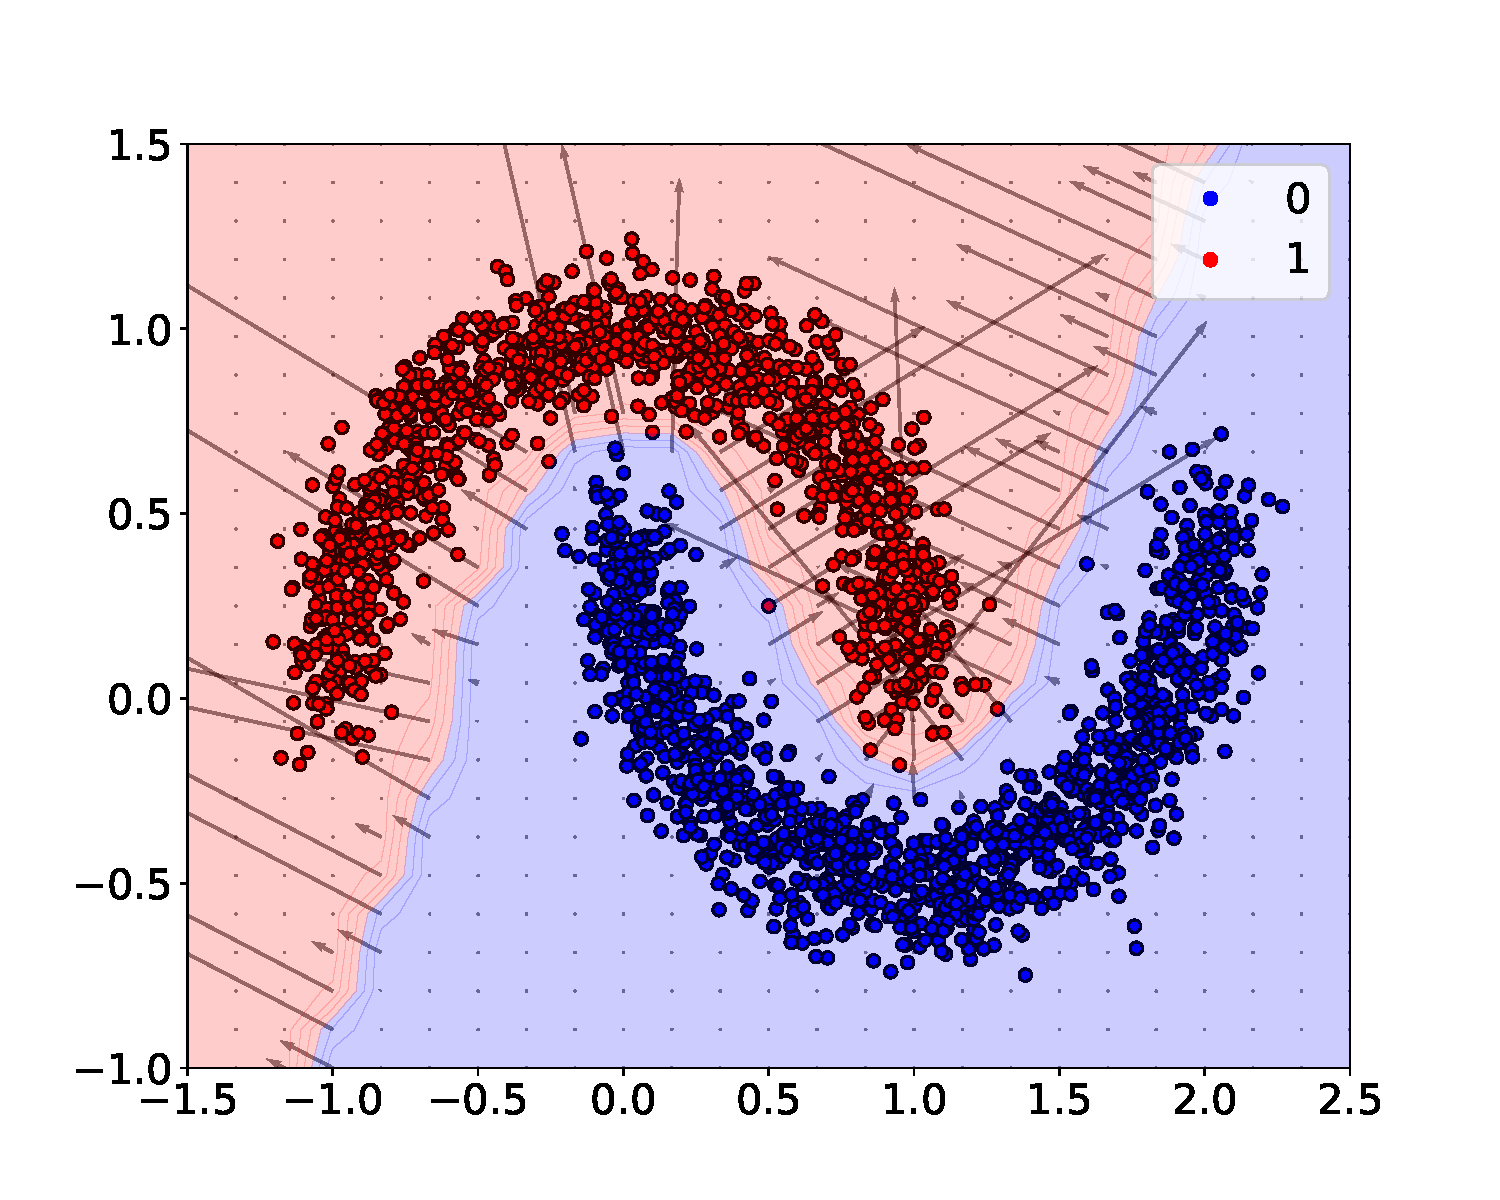
\includegraphics[width=0.9\columnwidth]{figures/half_moons.pdf}}
\caption{\textbf{Half moons dataset} with Gaussian noise $\mathcal{N}(0, 0.1)$. Predictions of an MLP are illustrated in blue and red colours. The gradient field of the model is represented by gray arrows. We can see that, as expected, the gradients are very high right on the decision boundary. However, they drop off to nearly zero everywhere else. The regions on each side of the decision boundary are shaded with different colours. The accuracy on the test set for this model is 99.9\%.}
\label{fig:half_moons}
\end{center}
\vskip -0.3in
\end{figure}

We now compute Integrated Gradients, Eq. \ref{eq:igi}, for this model on the test data. Let us consider a baseline and input pair, such that the baseline is outside of either half-moon, for example at (-0.5, -0.5). This is a good choice of baseline, since network should assign near-zero score to it. Let us call the feature in the vertical axis the $1$st component of $x$. In Fig. \ref{fig:ig} we illustrate the attribution of this feature, $IG_1(\textbf{x})$, for each point using the colour map. One should expect to see all the points sufficiently above the decision boundary to receive equally high attributions. Intuitively, this is expected, because if a point is above the decision boundary, its $x_1$ component is an important factor in the classification. However, for a model that is very skillful at the classification task, since the point is significantly above the decision boundary, going slightly down should not make any difference. Because in such a model's score should not change significantly anywhere other than near the decision boundary. However, we can see in Fig. \ref{fig:ig} that some points on the upper moon receive much higher $x_1$-attribution than others. These are points such that a straight line from the baseline to them mostly falls on high gradient regions. This does not reflect the model's behaviour. A similar point could be made about the horizontal axis. This is in contrast with Fig. \ref{fig:geodesic_ig}, where we show our method gives equally high attribution to all points sufficiently above the decision boundary, with different shades for the points closer to the boundary in $x_1$ direction. In Section \ref{subsec:half-moons} we present the details of how our method that achieves the results presented in this figure.

\begin{figure}[ht]
\vskip -0.1in
\begin{center}
\centerline{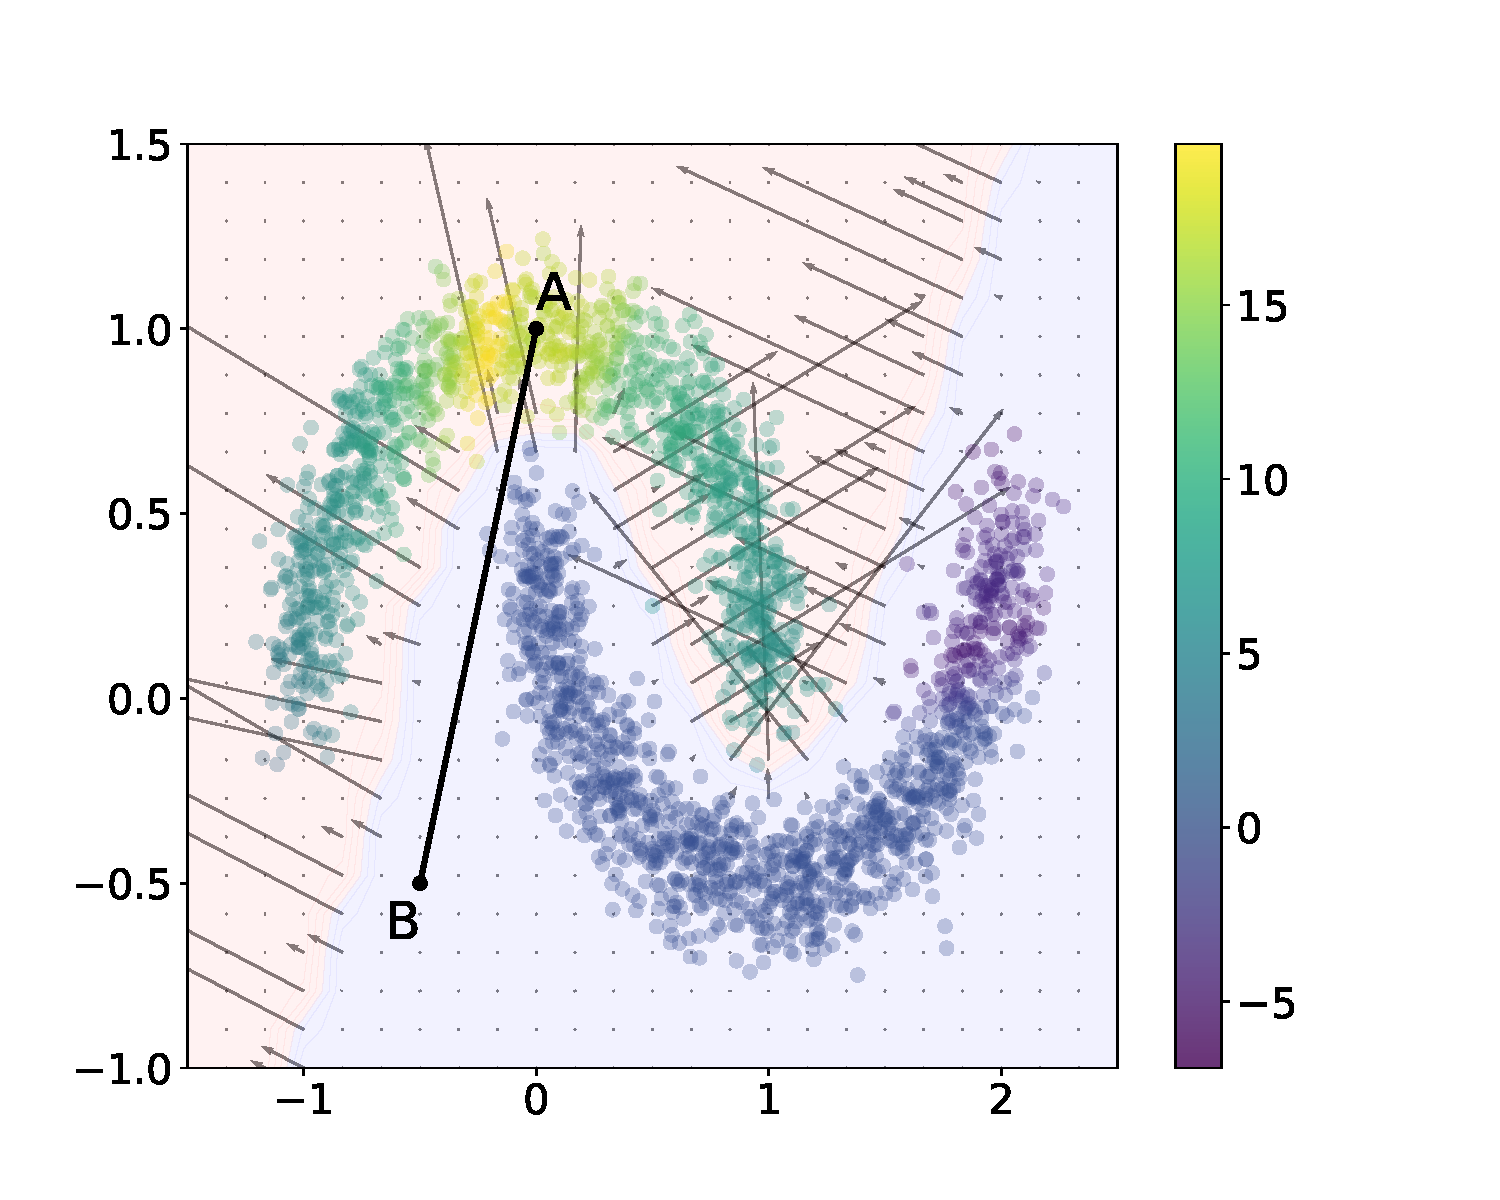
\includegraphics[width=\columnwidth]{figures/integrated_gradients_y.pdf}}
\vskip -0.2in
\caption{\textbf{Integrated Gradients attributions.} The colour map represents $\textrm{IG}_1(\textbf{x})$ for each point $\textbf{x}$, with $(-0.5, -0.5)$ (point B) as the baseline. Points around $A$ have much higher attributions than other points on the top moon, despite all being sufficiently above the decision boundary of the MLP. This is due to the path being close to the decision boundary, resulting in high gradients (gray arrows) along this path.}
\label{fig:ig}
\end{center}
\vskip -0.2in
\end{figure}

Before giving the formal method in section \ref{sec:method}, let us discuss the intuition behind our Geodesic IG. We want the path in Eq. \ref{eq:igi} to be such that it avoids regions with high model gradient. This is because failing to do so would superficially increase the result of the integral, leading to the types of artefacts illustrated in Fig. \ref{fig:ig}. Therefore, we should try to find the path of least resistance, as this is the path that avoids steep gradients as much as possible. As we shall see in section \ref{sec:method}, the input space can be viewed as a Riemannian manifold with a metric derived from the model gradients. The path of least resistance between a chosen baseline and input, therefore, is the geodesic path between the two points.

\begin{figure}[h!]
\vskip 0.2in
\begin{center}
\centerline{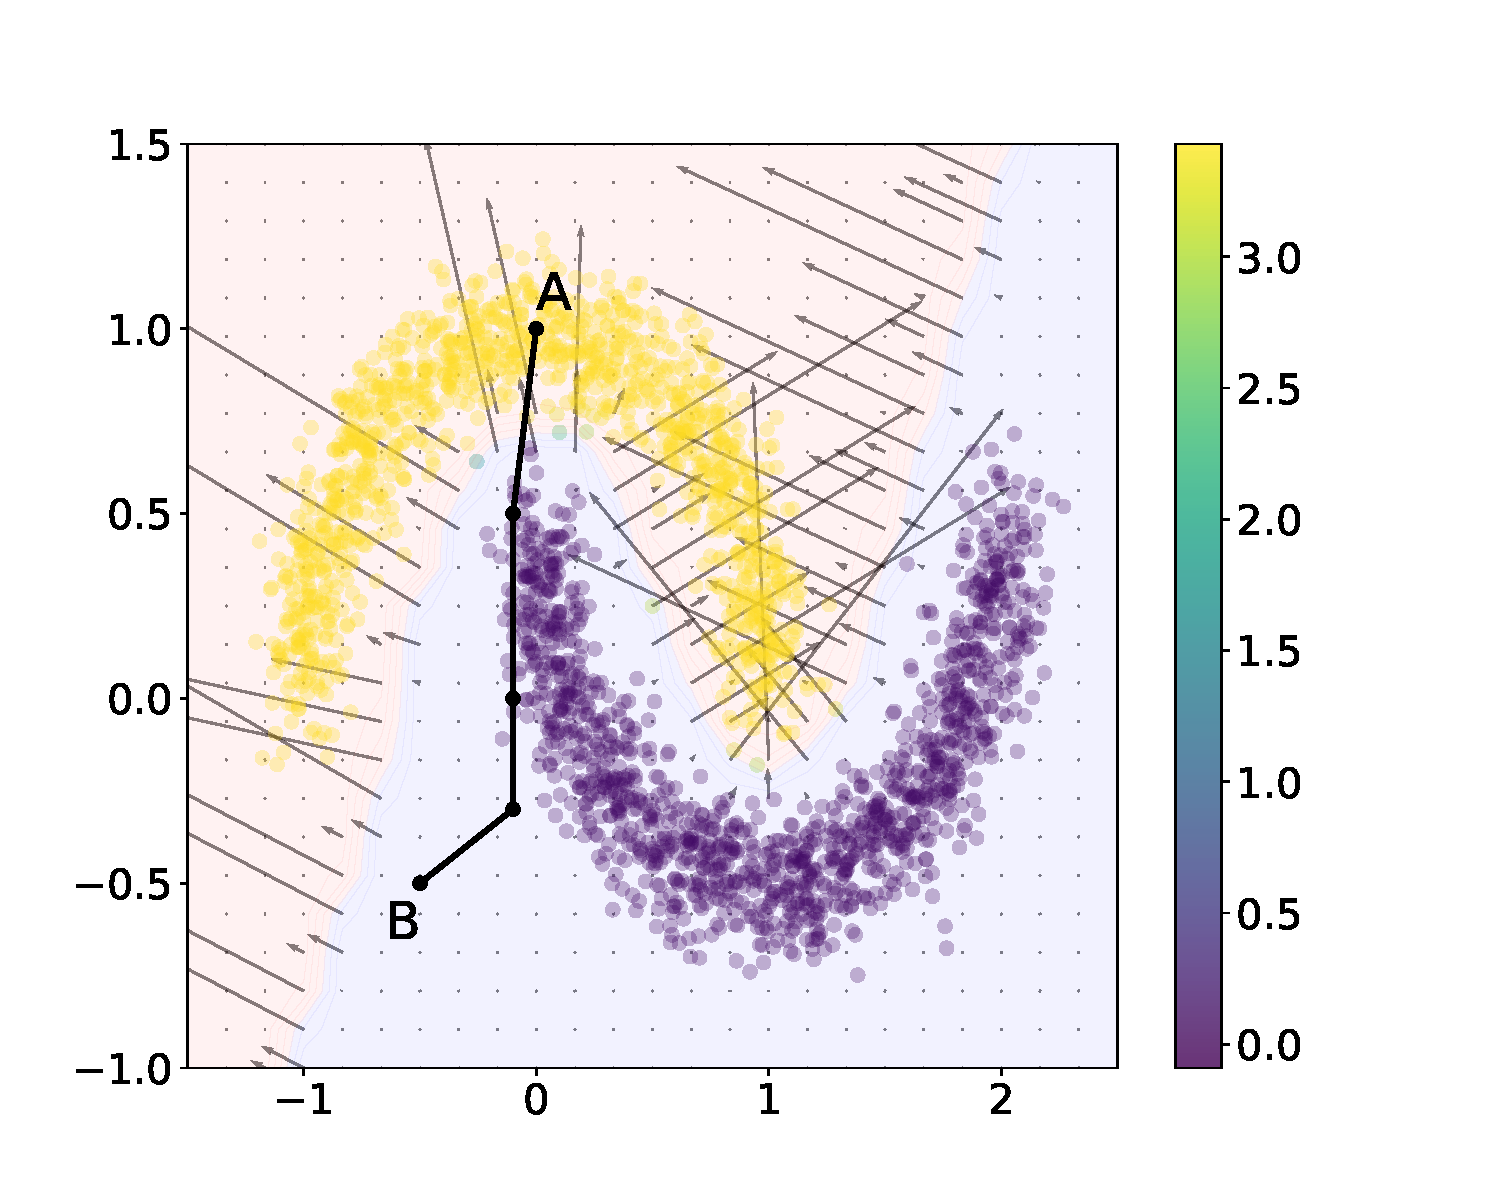
\includegraphics[width=\columnwidth]{figures/geodesic_ig_y.pdf}}
\caption{\textbf{Geodesic IG attributions.} Geodesic IG successfully avoids high gradients regions, and presents as a result attributions free of any artefacts. Moreover, unlike IG, there is no high variation of attributions between close points. We provide a rigorous comparison of Geodesic IG against various baselines in the Experiment section.}
\label{fig:geodesic_ig}
\end{center}
\vskip -0.2in
\end{figure}

In section \ref{sec:method}, we also develop a method to approximate the geodesic path between two points on the manifold to make solving the problem computationally feasible. We then show that geodesic IG satisfies all the axioms of IG, including symmetry. The symmetry axiom is defined in the following way. 
\begin{definition}
Consider an input-baseline pair $\textbf{x}$ and $\overline{\textbf{x}}$, and a function $f$ that is symmetric in dimensions $i$ and $j$. If $\textbf{x}_i = \textbf{x}_j$ and $\overline{\textbf{x}}_i = \overline{\textbf{x}}_j$, then an attribution method is Symmetry-Preserving if $attr_i(\textbf{x}; f) = attr_j(\textbf{x}; f)$, where $attr_n(\textbf{x}; f)$ is the attribution of $\textbf{x}_n$.
\end{definition}
\citep[Theorem 1]{sundararajan2017axiomatic} shows that IG is the only path method that satisfies symmetry on Euclidean space. We generalise this theorem for Geodesic IG on Riemannian manifolds.

In Section \ref{sec:experiments}, we demonstrate the effectiveness of the Geodesic IG method on the real-world Pascal VOC 2012 dataset \citep{pascal-voc-2012}. Our results outperform existing methods, as we evaluate using various metrics. We also provide supplementary experiments and and ablation studies in the appendix.

Section \ref{sec:related_work} reviews related work, including the comparison of Geodesic IG with other methods that attempt to overcome the shortcomings of Integrated Gradients.